% ---------------------------------------------------------------
% ---------------------------------------------------------------
% This template was developed for the working paper series of 
% the Interdisciplinary Laboratory of Computational Social Science (iLCSS)
% at the University of Maryland, College Park

% The template was built based on  the PNAS Latex model. 

% Adjustments were made by Tiago Ventura, Ph.D. Student in Political Science at UMD, 
% and researcher at the iLCSS.

\documentclass[9pt,twocolumn,twoside]{ilcss}
\usepackage{listings}
\usepackage[toc,page]{appendix}


\templatetype{ilcssworkingpaper} % Choose template 

\title{Un enfoque bayesiano para el análisis del tiempo de desplazamiento de usuarios del sistema de bicicletas públicas de la Ciudad de México}	

% Use letters for affiliations, numbers to show equal authorship (if applicable) and to indicate the corresponding author
\author[a]{Laura Gómez Bustamante}
\author[a]{Elizabeth Rodríguez Sánchez}
\author[a]{Miguel Ángel Millán Dorado}
\author[a]{C\'esar Zamora Mart\'inez}
%\author[b,1,2]{Author Two} 
%\author[a]{Author Three}

\affil[a]{Alumnos de Maestría en Ciencias de Datos (ITAM)}
%\affil[b]{Affiliation Two}
%\affil[c]{Affiliation Three}

% Please give the surname of the lead author for the running footer
\leadauthor{C\'esar Zamora Mart\'inez} 

% Please add here a significance statement to explain the relevance of your work
%\significancestatement{Authors must submit a 120-word maximum statement about the significance of their research paper written at a level understandable to an undergraduate educated scientist outside their field of speciality. The primary goal of the Significance Statement is to explain the relevance of the work in broad context to a broad readership. The Significance Statement appears in the paper itself and is required for all research papers.}

% Please include corresponding author, author contribution and author declaration information
%\authorcontributions{Please provide details of author contributions here.}
%\authordeclaration{Please declare any conflict of interest here.}
%\equalauthors{\textsuperscript{1}A.O.(Author One) and A.T. (Author Two) contributed equally to this work (remove if not applicable).}
\correspondingauthor{\textsuperscript{2}E-mail: czamora5\@email.itam.mx}

% Keywords are not mandatory, but authors are strongly encouraged to provide them. If provided, please include two to five keywords, separated by the pipe symbol, e.g:
%\keywords{Aprendizaje de Máquina $|$ Banda Ancha $|$ Telecomunicaciones $|$ ITAM} 

\begin{abstract}En fechas recientes el sistema de bicicletas públicas de la Ciudad de México (Ecobicis) ha ido ganando terreno como una opción que complementa el abanico de medios de transporte. 
\end{abstract}

%\dates{This manuscript was compiled on \today}

% You can change the link on the footer here

%\doi{\url{http://ilcss.umd.edu/}}

\begin{document}

\maketitle
\thispagestyle{firststyle}
\ifthenelse{\boolean{shortarticle}}{\ifthenelse{\boolean{singlecolumn}}{\abscontentformatted}{\abscontent}}{}

% If your first paragraph (i.e. with the \dropcap) contains a list environment (quote, quotation, theorem, definition, enumerate, itemize...), the line after the list may have some extra indentation. If this is the case, add \parshape=0 to the end of the list environment.

\dropcap{D}ada la compleja naturaleza de la movilidad 

l sistema de bicicletas públicas de la Ciudad de México ha sido adoptado por habitantes y turistas, debido a que este modo de transporte es la mejor opción para recorrer distancias cortas y medianas. Actualmente, ECOBICI cuenta con 480 cicloestaciones en 55 colonias de la ciudad, así como 6,800 bicicletas.

Usar ECOBICI es el complemento ideal con otros modos de transporte, lo que contribuye a mejorar la salud de los usuarios, la calidad de aire, entre otros.

Desde febrero de 2010, ECOBICI ha evolucionado paulatinamente. Hoy, cuenta con un sistema de bicicletas eléctricas de pedaleo asistido, que permite a los usuarios recorrer distancias más largas, con menor esfuerzo.

Estas bicicletas están disponibles en todo el polígono del sistema, cuya extensión actual es de 38 km2.

Por eso y más, ECOBICI es la manera inteligente de moverse.



\section{Revisión y análisis de fuentes de datos asociados a banda ancha fija}

hola

\subsection{Revisión de fuentes de información}

hola
\subsubsection{Identificación de municipios}

hola

\begin{table}[tbhp]
 \centering
	\caption{Distribución de accesos de BAF por tecnología (Junio 2019)\label{table:distribaccesosgrupos}}
	\begin{tabular}{@{}llllll@{}}
		\toprule
		Grupo & Coaxial & DSL & Fibra & Satelital & No especificado \\ \midrule
		América Móvil &  & 71.9\% & 28.1\% &  &  \\ 
		Grupo Televisa & 95.6\% &  &  & 0.1\% & 4.3\% \\ 
		Megacable-MCM & 99.9\% &  &  &  & 0.1\% \\ 
		TotalPlay &  &  & 100\% &  &  \\ \bottomrule
	\end{tabular}
\end{table}


\subsection{Conclusiones}

En este documento, exploramos el uso de modelos 
\bibliography{ilcss-sample}

\begin{appendices}
	
	\section{Repositorio Github}
	
	El desarrollo de este trabajo se consolidó a través de un repositorio en Github de acceso público: https://github.com/czammar/BandaAnchaFija; este contiene la totalidad de script desarrollados en Bash, R, Python, los mapas interactivos, las versiones en .tex de los documentos así como los datos empleados.
	
	\section{Figuras de análisis exploratorio}

\begin{figure}[tbhp]
	\centering
	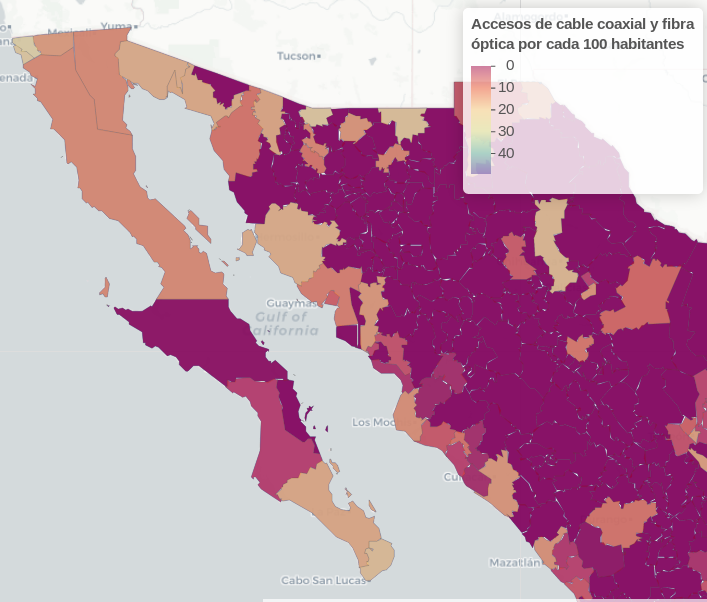
\includegraphics[width=0.9\linewidth]{images/pen_habs_penbc.png}
	\caption{Penetración de cable coaxial y fibra en la península de Baja California}
	\label{fig:pen_habs_penbc}
\end{figure}
\end{appendices}

\end{document}